% ------------------------------------------------------------
% LaTeX Template für die DHBW zum Schnellstart!
% Original: https://github.wdf.sap.corp/vtgermany/LaTeX-Template-DHBW
% ------------------------------------------------------------
% ---- Präambel mit Angaben zum Dokument
\documentclass[
	fontsize=12pt,           % Leitlinien sprechen von Schriftgröße 12.
	paper=A4,
	twoside=false,
	listof=totoc,            % Tabellen- und Abbildungsverzeichnis ins Inhaltsverzeichnis
	bibliography=totoc,      % Literaturverzeichnis ins Inhaltsverzeichnis aufnehmen
	titlepage,               % Titlepage-Umgebung anstatt \maketitle
	headsepline,             % horizontale Linie unter Kolumnentitel
	abstract,              % Überschrift einschalten, Abstract muss in {abstract}-Umgebung stehen
]{scrreprt}                  % Verwendung von KOMA-Report
\usepackage[utf8]{inputenc}  % UTF8 Encoding einschalten
\usepackage[ngerman]{babel}  % Neue deutsche Rechtschreibung
\usepackage[T1]{fontenc}     % Ausgabe von westeuropäischen Zeichen (auch Umlaute)
\usepackage{microtype}       % Trennung von Wörtern wird besser umgesetzt
\usepackage{lmodern}         % Nicht-gerasterte Schriftarten (bei MikTeX erforderlich)
\usepackage{graphicx}        % Einbinden von Grafiken erlauben
\usepackage{wrapfig}         % Grafiken fließend im Text
\usepackage{setspace}        % Zeilenabstand \singlespacing, \onehalfspaceing, \doublespacing
\usepackage[
	%showframe,                % Ränder anzeigen lassen
	left=2.7cm, right=2.5cm,
	top=2.5cm,  bottom=2.5cm,
	includeheadfoot
]{geometry}                      % Seitenlayout einstellen
\usepackage{scrlayer-scrpage}    % Gestaltung von Fuß- und Kopfzeilen
\usepackage{acronym}             % Abkürzungen, Abkürzungsverzeichnis
\usepackage{titletoc}            % Anpassungen am Inhaltsverzeichnis
\contentsmargin{0.75cm}          % Abstand im Inhaltsverzeichnis zw. Punkt und Seitenzahl
\usepackage[                     % Klickbare Links (enth. auch "nameref", "url" Package)
  hidelinks,                     % Blende die "URL Boxen" aus.
  breaklinks=true                % Breche zu lange URLs am Zeilenende um
]{hyperref}
\usepackage[hypcap=true]{caption}% Anker Anpassung für Referenzen
\urlstyle{same}                  % Aktuelle Schrift auch für URLs
% Anpassung von autoref für Gleichungen (ergänzt runde Klammern) und Algorithm.
% Anstatt "Listing" kann auch z.B. "Code-Ausschnitt" verwendet werden. Dies sollte
% jedoch synchron gehalten werden mit \lstlistingname (siehe weiter unten).
\addto\extrasngerman{%
	\def\equationautorefname~#1\null{Gleichung~(#1)\null}
	\def\lstnumberautorefname{Zeile}
	\def\lstlistingautorefname{Listing}
	\def\algorithmautorefname{Algorithmus}
	% Damit einheitlich "Abschnitt 1.2[.3]" verwendet wird und nicht "Unterabschnitt 1.2.3"
	% \def\subsectionautorefname{Abschnitt}
}

% ---- Abstand verkleinern von der Überschrift 
\renewcommand*{\chapterheadstartvskip}{\vspace*{.5\baselineskip}}

% Hierdurch werden Schusterjungen und Hurenkinder vermieden, d.h. einzelne Wörter
% auf der nächsten Seite oder in einer einzigen Zeile.
% LaTeX kann diese dennoch erzeugen, falls das Layout ansonsten nicht umsetzbar ist.
% Diese Werte sind aber gute Startwerte.
\widowpenalty10000
\clubpenalty10000

% ---- Für das Quellenverzeichnis
\usepackage[
	backend = biber,                % Verweis auf biber
	language = auto,
	style = numeric,                % Nummerierung der Quellen mit Zahlen
	sorting = none,                 % none = Sortierung nach der Erscheinung im Dokument
	sortcites = true,               % Sortiert die Quellen innerhalb eines cite-Befehls
	block = space,                  % Extra Leerzeichen zwischen Blocks
	hyperref = true,                % Links sind klickbar auch in der Quelle
	%backref = true,                % Referenz, auf den Text an die zitierte Stelle
	bibencoding = auto,
	giveninits = true,              % Vornamen werden abgekürzt
	doi=false,                      % DOI nicht anzeigen
	isbn=false,                     % ISBN nicht anzeigen
    alldates=short                  % Datum immer als DD.MM.YYYY anzeigen
]{biblatex}
\addbibresource{Inhalt/literatur.bib}
\setcounter{biburlnumpenalty}{3000}     % Umbruchgrenze für Zahlen
\setcounter{biburlucpenalty}{6000}      % Umbruchgrenze für Großbuchstaben
\setcounter{biburllcpenalty}{9000}      % Umbruchgrenze für Kleinbuchstaben
\DeclareNameAlias{default}{family-given}  % Nachname vor dem Vornamen
\AtBeginBibliography{\renewcommand{\multinamedelim}{\addslash\space
}\renewcommand{\finalnamedelim}{\multinamedelim}}  % Schrägstrich zwischen den Autorennamen
\DefineBibliographyStrings{german}{
  urlseen = {Einsichtnahme:},                      % Ändern des Titels von "besucht am"
}
\usepackage[babel,german=quotes]{csquotes}         % Deutsche Anführungszeichen + Zitate


% ---- Für Mathevorlage
\usepackage{amsmath}    % Erweiterung vom Mathe-Satz
\usepackage{amssymb}    % Lädt amsfonts und weitere Symbole
\usepackage{MnSymbol}   % Für Symbole, die in amssymb nicht enthalten sind.


% ---- Für Quellcodevorlage
\usepackage{scrhack}                    % Hack zur Verw. von listings in KOMA-Script
\usepackage{listings}                   % Darstellung von Quellcode
\usepackage{xcolor}                     % Einfache Verwendung von Farben
%% -- Eigene Farben für den Quellcode
\definecolor{JavaLila}{rgb}{0.4,0.1,0.4}
\definecolor{JavaGruen}{rgb}{0.3,0.5,0.4}
\definecolor{JavaBlau}{rgb}{0.0,0.0,1.0}
\definecolor{ABAPKeywordsBlue}{HTML}{6000ff}
\definecolor{ABAPCommentGrey}{HTML}{808080}
\definecolor{ABAPStringGreen}{HTML}{4da619}
\definecolor{PyKeywordsBlue}{HTML}{0000AC}
\definecolor{PyCommentGrey}{HTML}{808080}
\definecolor{PyStringGreen}{HTML}{008080}
% -- Farben für ABAP CDS
\definecolor{CDSString}{HTML}{FF8C00}
\definecolor{CDSKeywords}{HTML}{6000ff}
\definecolor{CDSAnnotation}{HTML}{00BFFF}
\definecolor{CDSComment}{HTML}{808080}
\definecolor{CDSFunc}{HTML}{FF0000}

% -- Default Listing-Styles

\lstset{
	% Das Paket "listings" kann kein UTF-8. Deswegen werden hier 
	% die häufigsten Zeichen definiert (ä,ö,ü,...)
	literate=%
		{á}{{\'a}}1 {é}{{\'e}}1 {í}{{\'i}}1 {ó}{{\'o}}1 {ú}{{\'u}}1
		{Á}{{\'A}}1 {É}{{\'E}}1 {Í}{{\'I}}1 {Ó}{{\'O}}1 {Ú}{{\'U}}1
		{à}{{\`a}}1 {è}{{\`e}}1 {ì}{{\`i}}1 {ò}{{\`o}}1 {ù}{{\`u}}1
		{À}{{\`A}}1 {È}{{\'E}}1 {Ì}{{\`I}}1 {Ò}{{\`O}}1 {Ù}{{\`U}}1
		{ä}{{\"a}}1 {ë}{{\"e}}1 {ï}{{\"i}}1 {ö}{{\"o}}1 {ü}{{\"u}}1
		{Ä}{{\"A}}1 {Ë}{{\"E}}1 {Ï}{{\"I}}1 {Ö}{{\"O}}1 {Ü}{{\"U}}1
		{â}{{\^a}}1 {ê}{{\^e}}1 {î}{{\^i}}1 {ô}{{\^o}}1 {û}{{\^u}}1
		{Â}{{\^A}}1 {Ê}{{\^E}}1 {Î}{{\^I}}1 {Ô}{{\^O}}1 {Û}{{\^U}}1
		{œ}{{\oe}}1 {Œ}{{\OE}}1 {æ}{{\ae}}1 {Æ}{{\AE}}1 {ß}{{\ss}}1
		{ű}{{\H{u}}}1 {Ű}{{\H{U}}}1 {ő}{{\H{o}}}1 {Ő}{{\H{O}}}1
		{ç}{{\c c}}1 {Ç}{{\c C}}1 {ø}{{\o}}1 {å}{{\r a}}1 {Å}{{\r A}}1
		{€}{{\euro}}1 {£}{{\pounds}}1 {«}{{\guillemotleft}}1
		{»}{{\guillemotright}}1 {ñ}{{\~n}}1 {Ñ}{{\~N}}1 {¿}{{?`}}1,
	breaklines=true,        % Breche lange Zeilen um 
	breakatwhitespace=true, % Wenn möglich, bei Leerzeichen umbrechen
	% Symbol für Zeilenumbruch einfügen
	prebreak=\raisebox{0ex}[0ex][0ex]{\ensuremath{\rhookswarrow}},
	postbreak=\raisebox{0ex}[0ex][0ex]{\ensuremath{\rcurvearrowse\space}},
	tabsize=4,                                 % Setze die Breite eines Tabs
	basicstyle=\ttfamily\small,                % Grundsätzlicher Schriftstyle
	columns=fixed,                             % Besseres Schriftbild
	numbers=left,                              % Nummerierung der Zeilen
	%frame=single,                             % Umrandung des Codes
	showstringspaces=false,                    % Keine Leerzeichen hervorheben
	keywordstyle=\color{blue},
	ndkeywordstyle=\bfseries\color{darkgray},
	identifierstyle=\color{black},
	commentstyle=\itshape\color{JavaGruen},   % Kommentare in eigener Farbe
	stringstyle=\color{JavaBlau},             % Strings in eigener Farbe,
	captionpos=b,                             % Bild*unter*schrift
	xleftmargin=5.0ex
}

% ---- Eigener JAVA-Style für den Quellcode
\renewcommand{\ttdefault}{pcr}               % Schriftart, welche auch fett beinhaltet
\lstdefinestyle{EigenerJavaStyle}{
	language=Java,                             % Syntax Highlighting für Java
	%frame=single,                             % Umrandung des Codes
	keywordstyle=\bfseries\color{JavaLila},    % Keywords in eigener Farbe und fett
	commentstyle=\itshape\color{JavaGruen},    % Kommentare in eigener Farbe und italic
	stringstyle=\color{JavaBlau}               % Strings in eigener Farbe
}

% ---- Eigener ABAP-Style für den Quellcode
\renewcommand{\ttdefault}{pcr}
\lstdefinestyle{EigenerABAPStyle}{
	language=[R/3 6.10]ABAP,
	morestring=[b]\|,                          % Für Pipe-Strings
	morestring=[b]\`,                          % für Backtick-Strings
	keywordstyle=\bfseries\color{ABAPKeywordsBlue},
	commentstyle=\itshape\color{ABAPCommentGrey},
	stringstyle=\color{ABAPStringGreen},
	tabsize=2,
	morekeywords={
		types,
		@data,
		as,
		lower,
		start,
		selection,
		order,
		by,
		inner,
		join,
		key,
		end,
		cast
	}
}

% ---- Eigener Python-Style für den Quellcode
\renewcommand{\ttdefault}{pcr}
\lstdefinestyle{EigenerPythonStyle}{
	language=Python,
	columns=flexible,
	keywordstyle=\bfseries\color{PyKeywordsBlue},
	commentstyle=\itshape\color{PyCommentGrey},
	stringstyle=\color{PyStringGreen}
}

%----- ABAP-CDS-View language
\lstdefinelanguage{ABAPCDS}{
	sensitive=false,
	%Keywords
	morekeywords={define,
		view,
		as,
		select,
		from,
		inner,
		join,
		on,
		key,
		case,
		when,
		then,
		else,
		end,
		true,
		false,
		cast,
		where,
		and,
		distinct,
		group,
		by,
		having,
		min,
		sum,
		max,
		count,
		avg
	},
	%Methoden
	morekeywords=[2]{
		div,
		currency\_conversion,
		dats\_days\_between,
		concat\_with\_space,
		dats\_add_days,
		dats\_is\_valid,
		dats\_add\_months,
		unit\_conversion,
		division,
		mod,
		abs,
		floor,
		ceil,
		round,
		concat,
		replace,
		substring,
		left,
		right,
		length
	},
	morecomment=[s][\color{CDSAnnotation}]{@}{:},
	morecomment=[l][\itshape\color{CDSComment}]{//},
	morecomment=[s][\itshape\color{CDSComment}]{/*}{*/},
	morestring=[b][\color{CDSString}]',
	keywordstyle=\bfseries\color{CDSKeywords},
	keywordstyle=[2]\color{CDSFunc}
}

  % Weitere Details sind ausgelagert

\usepackage{algorithm}                  % Für Algorithmen-Umgebung (ähnlich wie lstlistings Umgebung)
\usepackage{algpseudocode}              % Für Pseudocode. Füge "[noend]" hinzu, wenn du kein "endif",
                                        % etc. haben willst.

\makeatletter                           % Sorgt dafür, dass man @ in Namen verwenden kann.
                                        % Ansonsten gibt es in der nächsten Zeile einen Compilefehler.
\renewcommand{\ALG@name}{Algorithmus}   % Umbenennen von "Algorithm" im Header der Listings.
\makeatother                            % Zeichen wieder zurücksetzen
\renewcommand{\lstlistingname}{Listing} % Erlaubt das Umbenennen von "Listing" in anderen Titel.

% ---- Tabellen
\usepackage{booktabs}  % Für schönere Tabellen. Enthält neue Befehle wie \midrule
\usepackage{multirow}  % Mehrzeilige Tabellen
\usepackage{siunitx}   % Für SI Einheiten und das Ausrichten Nachkommastellen
\sisetup{locale=DE, range-phrase={~bis~}, output-decimal-marker={,}} % Damit ein Komma und kein Punkt verwendet wird.
\usepackage{xfrac} % Für siunitx Option "fraction-function=\sfrac"
\usepackage{hyperref} %teststetststsstst

% ---- Für Definitionsboxen in der Einleitung
\usepackage{amsthm}                     % Liefert die Grundlagen für Theoreme
\usepackage[framemethod=tikz]{mdframed} % Boxen für die Umrandung
%% ---- Definition für Highlight Boxen

% ---- Grundsätzliche Definition zum Style
\newtheoremstyle{defi}
  {\topsep}         % Abstand oben
  {\topsep}         % Abstand unten
  {\normalfont}     % Schrift des Bodys
  {0pt}             % Einschub der ersten Zeile
  {\bfseries}       % Darstellung von der Schrift in der Überschrift
  {:}               % Trennzeichen zwischen Überschrift und Body
  {.5em}            % Abstand nach dem Trennzeichen zum Body Text
  {\thmname{#3}}    % Name in eckigen Klammern
\theoremstyle{defi}

% ------ Definition zum Strich vor eines Texts
\newmdtheoremenv[
  hidealllines = true,       % Rahmen komplett ausblenden
  leftline = true,           % Linie links einschalten
  innertopmargin = 0pt,      % Abstand oben
  innerbottommargin = 4pt,   % Abstand unten
  innerrightmargin = 0pt,    % Abstand rechts
  linewidth = 3pt,           % Linienbreite
  linecolor = gray!40,       % Linienfarbe
]{defStrich}{Definition}     % Name der des formats "defStrich"

% ------ Definition zum Eck-Kasten um einen Text
\newmdtheoremenv[
  hidealllines = true,
  innertopmargin = 6pt,
  linecolor = gray!40,
  singleextra={              % Eck-Markierungen für die Definition
    \draw[line width=3pt,gray!50,line cap=rect] (O|-P) -- +(1cm,0pt);
    \draw[line width=3pt,gray!50,line cap=rect] (O|-P) -- +(0pt,-1cm);
    \draw[line width=3pt,gray!50,line cap=rect] (O-|P) -- +(-1cm,0pt);
    \draw[line width=3pt,gray!50,line cap=rect] (O-|P) -- +(0pt,1cm);
  }
]{defEckKasten}{Definition}  % Name der des formats "defEckKasten"  % Weitere Details sind ausgelagert

% ---- Für Todo Notes
\usepackage{todonotes}
\setlength {\marginparwidth }{2cm}      % Abstand für Todo Notizen

% ---- Zum Einbinden von PDF-Dokumenten
\usepackage{pdfpages}


% ---- Elektronische Version oder Gedruckte Version?
% ---- Unterschied: Die elektronische Version enthält keinen Platzhalter für die Unterschrift
\usepackage{ifthen}
\newboolean{e-Abgabe}
\setboolean{e-Abgabe}{false}    % false=gedruckte Fassung

% ---- Persönlichen Daten:
\newcommand{\titel}{Emissionszertifikate als umweltpolitisches Instrument gegen den Klimawandel: Theorie und Praxis}
\newcommand{\titelheader}{Emissionszertifikate}
\newcommand{\arbeit}{Seminararbeit VWL 2}
\newcommand{\studiengang}{Wirtschaftsinformatik Software Engineering}
\newcommand{\studienjahr}{2022}
\newcommand{\autor}{Alexander Meinecke}
\newcommand{\autorReverse}{Meinecke, Alexander}
\newcommand{\verfassungsort}{Mannheim}
\newcommand{\matrikelnr}{1522347}
\newcommand{\kurs}{WWI22SEB}
\newcommand{\bearbeitungsmonat}{Dezember 2023}
\newcommand{\abgabe}{25. Januar 2024}
\newcommand{\bearbeitungszeitraum}{Dezember 2023 - 25. Januar 2024}
\newcommand{\firmaName}{SAP SE}
\newcommand{\firmaStrasse}{Dietmar-Hopp-Allee 16}
\newcommand{\firmaPlz}{69190 Walldorf, Deutschland}
\newcommand{\betreuerDhbw}{Prof. Dr. Frank Hubert}

% ---- Metainformation für das PDF Dokument
\hypersetup{
	pdftitle    = {\titel},
	pdfsubject  = {\arbeit},
	pdfauthor   = {\autor},
	%pdfkeywords = {Keywords angeben},
	pdfcreator  = {LaTeX},
	%pdfproducer = {in der Regel pdfTeX}
}

% ---- Definition der Kopf- und Fußzeilen
\clearpairofpagestyles                          % Löschen von LaTeX Standard
\automark[section]{chapter}                     % Füllen von section und chapter
\renewcommand*{\chaptermarkformat}{}            % Entfernt die Kapitelnummer
\renewcommand*{\sectionmarkformat}{}            % Entfernt die Sectionnummer
% Angaben [für "plain"]{für "scrheadings"}
\ihead[]{\titelheader}                          % Kopfzeile links
\chead[]{}                                      % Kopfzeile mitte
\ohead[]{\rightmark}                            % Kopfzeile rechts
\ifoot[]{}                                      % Fußzeile links
\cfoot*{\sffamily\pagemark}                     % Fußzeile mitte
\ofoot[]{}                                      % Fußzeile rechts
\KOMAoptions{
   headsepline = 0.2pt,                         % Liniendicke Kopfzeile
   footsepline = false                          % Liniendicke Fußzeile
}


% ---- Hilfreiches
\newcommand{\zB}{z.\,B. }   % "z.B." mit kleinem Leeraum dazwischen (ohne wäre nicht korrekt)
\newcommand{\dash}{d.\,h. }

\newcommand{\code}[1]{\texttt{#1}} % Ist einfacher zu schreiben als ständig \texttt und erlaubt
                                   % Änderungen im Nachhinein, wenn man z.B. Inline-Code anders stylen möchte.

% ---- Silbentrennung (falls LaTeX defaults falsch / nicht gewünscht sind)
\hyphenation{HANA}         % anstatt HA-NA
\hyphenation{Graph-Script} % anstatt GraphS-cript

% ---- Beginn des Dokuments
\begin{document}
\setlength{\parindent}{0pt}              % Keine Paragraphen Einrückung.
                                         % Dafür haben wir den Abstand zwischen den Paragraphen.
\setcounter{secnumdepth}{2}              % Nummerierungstiefe fürs Inhaltsverzeichnis
\setcounter{tocdepth}{1}                 % Tiefe des Inhaltsverzeichnisses. Ggf. so anpassen,
                                         % dass das Verzeichnis auf eine Seite passt.
\sffamily                                % Serifenlose Schrift verwenden.

% ---- Vorspann
% ------ Titelseite
\singlespacing
\thispagestyle{empty}
\begin{titlepage}
\enlargethispage{4cm}

\begin{figure}           % Logo vom Ausbildungsbetrieb und der DHBW
	% \vspace*{-5mm} % Sollte dein Titel zu lang werden, kannst du mit diesem "Hack" 
	%                  den Inhalt der Seite nach oben schieben.
	\begin{minipage}{0.49\textwidth}
		\flushleft
		
\includegraphics[height=2.5cm]{Bilder/Logos/Logo_SAP.pdf} 
	\end{minipage}
	\hfill
	\begin{minipage}{0.49\textwidth}
		\flushright
		
\includegraphics[height=2.5cm]{Bilder/Logos/Logo_DHBW.pdf} 
	\end{minipage}
\end{figure} 
\vspace*{0.1cm}

\begin{center}
	\huge{\textbf{\titel}}\\[1.5cm]
	\Large{\textbf{\arbeit}}\\[0.5cm]
	\normalsize{im Rahmen der Prüfung zum\\[1ex] \textbf{Bachelor of Science (B.Sc.)}}\\[0.5cm]
	\Large{des Studienganges \studiengang}\\[1ex]
	\normalsize{an der Dualen Hochschule Baden-Württemberg Mannheim}\\[1cm]
	\normalsize{von}\\[1ex] \Large{\textbf{\autor}} \\[1cm]
	% Hinweis: Manche Dozenten möchten einen Hinweis auf den Sperrvermerk auf der Titelseite.
	% \large{{\color{red}- Sperrvermerk -}}\\[1cm]
\end{center}

\begin{center}
	\vfill
	\begin{tabular}{ll}
		Abgabedatum:                     & \abgabe \\[0.2cm]
		Bearbeitungszeitraum:            & \bearbeitungszeitraum \\[0.2cm]
		Matrikelnummer, Kurs:            & \matrikelnr , \kurs \\[0.2cm]
		Ausbildungsfirma:                & \firmaName \\
		                                 & \firmaStrasse \\
		                                 & \firmaPlz \\[0.2cm]
		
		Gutachter: 						& \betreuerDhbw \\[2cm]
	\end{tabular} 
\end{center}
\end{titlepage}
  % Titelseite
\newcounter{savepage}
\pagenumbering{Roman}                    % Römische Seitenzahlen
\onehalfspacing

% ------ Erklärung, Sperrvermerk, Abstact
\chapter*{Eidesstattliche Erklärung}
Ich versichere hiermit, dass ich meine \arbeit{} mit dem Thema:
\begin{quote}
	\textit{\titel}
\end{quote} 
gemäß § 5 der \enquote{Studien- und Prüfungsordnung DHBW Technik} vom 29. September 2017 selbstständig verfasst und keine anderen als die angegebenen Quellen und Hilfsmittel benutzt habe. Die Arbeit wurde bisher keiner anderen Prüfungsbehörde vorgelegt und auch nicht veröffentlicht.

\vspace{0.25cm}

Ich versichere zudem, dass die eingereichte elektronische Fassung mit der gedruckten Fassung übereinstimmt.

\vspace{1cm}

\verfassungsort, den \today \\[0.5cm]
\ifthenelse{\boolean{e-Abgabe}}
	{\underline{Gez. \autor}}
	{\makebox[6cm]{\hrulefill}}\\ 
\autorReverse

%\chapter*{Sperrvermerk}
Die nachfolgende Arbeit enthält vertrauliche Daten der:
\begin{quote}
	\firmaName \\
	\firmaStrasse \\
	\firmaPlz
\end{quote}

\vspace{0.5cm}

Der Inhalt dieser Arbeit darf weder als Ganzes noch in Auszügen Personen außerhalb des Prüfungsprozesses und des Evaluationsverfahrens zugänglich gemacht werden, sofern keine anderslautende Genehmigung vom Dualen Partner vorliegt.

%\renewcommand{\abstractname}{Abstract} % Veränderter Name für das Abstract
\begin{abstract}
\begin{addmargin}[1.5cm]{1.5cm}        % Erhöhte Ränder, für Abstract Look
\thispagestyle{plain}                  % Seitenzahl auf der Abstract Seite

\begin{center}
\small\textit{- English -}             % Angabe der Sprache für das Abstract
\end{center}

\vspace{0.25cm}

This is the starting point of the Abstract. For the final bachelor thesis, there must be an abstract included in your document. So, start now writing it in German and English. The abstract is a short summary with around 200 to 250 words.

\vspace{0.25cm}

Try to include in this abstract the main question of your work, the methods you used or the main results of your work.


\end{addmargin}
\end{abstract}
%\renewcommand{\abstractname}{Abstract} % Veränderter Name für das Abstract
\begin{abstract}
\begin{addmargin}[1.5cm]{1.5cm}        % Erhöhte Ränder, für Abstract Look
\thispagestyle{plain}                  % Seitenzahl auf der Abstract Seite

\begin{center}
\small\textit{- Deutsch -}             % Angabe der Sprache für das Abstract
\end{center}

\vspace{0.25cm}

Dies ist der Beginn des Abstracts. Für die finale Bachelorarbeit musst du ein Abstract in deinem Dokument mit einbauen. So, schreibe es am besten jetzt in Deutsch und Englisch. Das Abstract ist eine kurze Zusammenfassung mit ca. 200 bis 250 Wörtern.

\vspace{0.25cm}

Versuche in das Abstract folgende Punkte aufzunehmen: Fragestellung der Arbeit, methodische Vorgehensweise oder die Hauptergebnisse deiner Arbeit.


\end{addmargin}
\end{abstract}

% ------ Inhaltsverzeichnis
\singlespacing
\tableofcontents

% ------ Verzeichnisse
\renewcommand*{\chapterpagestyle}{plain}
\pagestyle{plain}
%\chapter*{Formelverzeichnis}
\addcontentsline{toc}{chapter}{Formelverzeichnis} % Hinzufügen zum Inhaltsverzeichnis 

% Definition des neuen Befehls für das Einfügen der Abkürzung der Einheit
\newcommand{\acrounit}[1]{
  \acroextra{\makebox[18mm][l]{\si[per-mode=fraction,fraction-function=\sfrac]{#1}}}
}
\begin{acronym}[dmin] % längstes Kürzel wird verw. für den Abstand zw. Kürzel u. Text

	% Alphabetisch selbst sortieren - nicht verwendete Formeln rausnehmen!
	% Allgemein: \acro{KÜRZEL}[ABKÜRZUNG]{\acrounit{SI-EINHEIT}BESCHREIBUNG}

	\acro{A}[\ensuremath{A}]{\acrounit{mm^2}Fläche}	
	\acro{D}[\ensuremath{D}]{\acrounit{mm}Werkstückdurchmesser}	
	\acro{dmin}[\ensuremath{d\textsubscript{min}}]{\acrounit{mm}kleinster Schaftdurchmesser}	
	\acro{L1}[\ensuremath{L\textsubscript{1}}]{\acrounit{mm}Länge des Werkstückes Nr. 1}	
	\acro{Fwinkel}[]{\acrounit{Grad}Freiwinkel}	
	\acro{Kwinkel}[]{\acrounit{Grad}Keilwinkel}

\end{acronym}

\listoffigures % Erzeugen des Abbildungsverzeichnisses 
\chapter*{Abkürzungsverzeichnis}
\addcontentsline{toc}{chapter}{Abkürzungsverzeichnis} % Hinzufügen zum Inhaltsverzeichnis 

\begin{acronym}[WYSISWG] % längstes Kürzel wird verw. für den Abstand zw. Kürzel u. Text

	% Alphabetisch selbst sortieren - nicht verwendete Kürzel rausnehmen!
	\acro{BEHG}{Brennstoffemissionshandelsgesetz}
	\acro{CBAM}{Carbon Border Adjustment Mechanism (dt. Grenzausgleichsmechanismus)}
	\acro{DEHSt}{Deutsche Emissionshandelsstelle}
	\acro{ETS}{Emission Trading System (dt. Emissionshandelssystem)}
	\acro{ICAP}{International Carbon Action Partnership (dt. Internationale Partnerschaft für Emissionshandel)}
	\acro{MSR}{Market Stability Reserve (dt. Marktstabilitätsreserve)}
	\acro{nEHS}{Nationales Emissionshandelssystem}
	\acro{TNAC}{Total Number of Allowances in Circulation (dt. Anzahl der Zertifikate im Umlauf)}

\end{acronym}           
%\listoftables                           % Erzeugen des Tabellenverzeichnisses
%\renewcommand{\lstlistlistingname}{Quellcodeverzeichnis}
%\lstlistoflistings                      % Erzeugen des Listenverzeichnisses
\setcounter{savepage}{\value{page}}


% ---- Inhalt der Arbeit
\cleardoublepage
\pagenumbering{arabic}                  % Arabische Seitenzahlen für den Hauptteil
\setlength{\parskip}{0.5\baselineskip}  % Abstand zwischen Absätzen
\rmfamily
\renewcommand*{\chapterpagestyle}{scrheadings}
\pagestyle{scrheadings}
\onehalfspacing
\chapter{Einleitung}

Der Klimawandel ist eine der größten Herausforderungen unserer Zeit. Um gegen Phänomen vorzugehen, müssen die Volkswirtschaften klimaneutral werden (vgl. \cite[S. 162]{hubert.2020}).
Doch das Recht, Treibhausgase zu emittieren, war lange Zeit kostenlos. Wenn für die Produktion eines Gutes Treibhausgase anfielen, wurde dies nicht bei der Preisfindung am Markt zwischen Anbieter und Nachfrager berücksichtigt (vgl. \cite[S. 161]{hubert.2020}).
Dabei entstehen bei der Emission von Treibhausgasen externe Kosten, die sich durch langfristige Wohlfahrtsverluste bemerkbar machen werden (vgl. \cite[S. 25]{rabe.2018}) (vgl. \cite{ub4.2023}).
Diese Kosten können z.B. in Form von Schäden durch Naturkatastrophen, Ernteausfällen oder durch den Anstieg des Meeresspiegels entstehen.
Das Umweltbundesamt geht bei einer Gleichgewichtung klimawandelverursachter Wohlfahrtseinbußen heutiger und zukünftiger Generationen von Kosten in Höhe von 809 Euro pro Tonne $CO_2$ aus (vgl. \cite{ub4.2023}).
Bei verfälschter Preisbildung am Markt wird auch von Marktversagen gesprochen (vgl. \cite[S. 268]{hubert.2019}).
Um die externen Mehrkosten von Treibhausgasen zu berücksichtigen und so die Fehlpreisbildung zu korrigieren, müssen diese in die Preisfindung am Markt internalisiert werden (vgl. \cite[S. 161]{hubert.2020}).

Es gibt verschiedene Lenkungsmöglichkeiten, die Staaten einsetzen können, um ihre Volkswirtschaften klimaneutral zu machen.
Neben einer $CO_2$-Steuer und Verhandlungslösungen nach dem Coase-Theorem gibt es das Konzept der Emissionshandelssysteme (vgl. \cite[S. 161]{hubert.2020}).
In dieser Seminararbeit wird Letzteres genauer in Theorie und Praxis betrachtet.
\chapter{Theorie}

Ein Emissionshandelssystem setzt auf das Verursacherprinzip \cite[S. 161]{hubert.2020}.
Das bedeutet, dass die Akteure, die tatsächlich für die Emissionen verantwortlich sind, in einer Volkswirtschaft monetär zur Verantwortung gezogen werden.
In einem Emissionshandelssystem werden die Rechte, Treibhausgase zu emittieren, als Zertifikate dargestellt \cite[S. 27]{rabe.2018}.
Ein Zertifikat berechtigt den Besitzer, eine Tonne CO2-Äquivalente (CO2e) zu emittieren.
Es wird von Äquivalenten gesprochen, da es neben CO2 verschiedene Treibhausgase gibt, die unterschiedlich stark zum Klimawandel beitragen. CO2 wird als Referenzgröße verwendet.
Es wird hier auch vom 'Global Warming Potential' gesprochen. So hat bspw. Methan ein 28-fach höheres Global Warming Potential als CO2 \cite{ub.2023}.
Stößt ein Verursacher mehr CO2e aus, als er Zertifikate besitzt, muss dieser hohe Sanktionszahlungen leisten, die in keinem Verhältnis zu den tatsächlichen 'Ersparnissen' durch den Nichtkauf der Zertifikate stehen und daher ökonomisch keinen Sinn machen \cite[S. 181]{hubert.2020}.

Das Kernkonzept eines Emissionshandelssystems ist das sog. 'Cap and Trade' (dt. 'Verknappen und Handeln') \cite[S. 134]{rabe.2018}.
Aus den Klimaschutzzielen einer Regierung wird eine Obergrenze (CAP) für die Emissionenzertifikate bis zu einem bestimmten Zeitpunkt festgelegt, also der Zeitpunkt, bis zu dem die Volkswirtschaft klimaneutral sein soll \cite[S. 181]{hubert.2020}.
Die Zertifikate unterhalb dieser Obergrenze werden nun jährlich entweder unter Orientierung an dem bisherigen Treibhausgasaustoß eines Verursachers kostenlos oder kostenpflichtig verteilt oder alternativ versteigert \cite[S. 181]{hubert.2020}.

Aus dem bislang öffentlichen Gut 'Emissionen ausstoßen' wird so durch die Obergrenze ein knappes Gut, mit dem nach der Ausgabe der Zertifikate somit marktwirtschaftlich gehandelt werden kann (Trade) \cite[S. 17]{hubert.2020}.
Anfangs werden noch verhältnismäßig viele Zertifikate ausgegeben, die Menge wird aber jährlich reduziert \cite[S. 182]{hubert.2020}. So steigt der Preis der Zertifikate an.
Verursacher, die mehr Zertifikate benötigen als sie erhalten haben, müssen diese von anderen Unternehmen kaufen \cite[S. 182]{hubert.2020}.
Andersherum können Verursacher Zertifikate verkaufen, die sie nicht benötigen.
So entsteht eine Lenkungswirkung, Unternehmen dazu zu bringen, weniger Treibhausgase zu emittieren und auf innovativere, klimaneutralere Technologien umzustellen.
Unternehmen, die sich nicht rechtzeitig reformieren, sind aufgrund der steigenden CO2e-Preise weniger wettbewerbsfähig und werden vom Markt verdrängt.
\chapter{Praxis}

Aktuell betreffen uns in Deutschland zwei kontrete Emissionshandelssysteme. Zum einen das EU-Emissionshandelssystem (ETS) und zum anderen das nationale Emissionshandelssystem (nEHS), das durch das Brennstoffemissionshandelsgesetz (BEHG) geregelt wurde.

\section{EU-Emissionshandelssystem (ETS)}

Das ETS ist das weltweit größte Emissionshandelssystem. Es wurde 2005 eingeführt und deckt ca. 40\% der Treibhausgasemissionen der EU ab. Das ETS gilt für den europäischen Binnenmarkt sowie für die Staaten Island, Lichtenstein und Norwegen. Sie zielt auf direkte Emissionen aus der produzierenden Industrie, dem Energiesektor und der Luftfahrt ab. Ab 2024 sind auch Emissionen aus der Schiffahrt vom ETS gedeckt \cite{eu.2023}.
Bei dem ETS handelt es sich um einen s.g. Downstream Emissionshandel. Das bedeutet, dass Emittenten die Berechtigung für ihre Emissionen selbst erwerben. Das bedeutet, dass die Emittenten von sich aus den Anreiz haben, ihre CO2e-Austoß zu senken.  
\chapter{Fazit}

Emissionshandelssysteme sind als marktwirtschaftliches Instrument gegen den Klimawandel einzigartig aufgrund ihrer ökologischen Treffsicherheit \cite[S. 182]{hubert.2020}.
Dies ist auf den sinkenden Emissions-Cap einer Volkswirtschaft zurückzuführen, mit dem die Menge der ausgestoßenen Treibhausgase kontrolliert werden kann.
Voraussetzung dafür ist, dass der Cap nicht zu hoch angesetzt wird, wie am Negativbeispiel der Zertifikatsmenge des EU ETS nach der Finanzkrise gesehen werden kann \cite{eu3.2023}.

Ein weiterer Vorteil ist die ökonomische Effizienz. Unternehmen und Verbraucher haben selbst die Wahl, wie sie ihre Emissionen reduzieren.
Sie können selbst entscheiden, wo sie Emissionen vermeiden wollen und wo nicht. Langfristig kann kein Verbraucher das Problem des Treibhausgasausstoßes ignorieren, da sonst die Kosten für seine Emissionen zu hoch werden.
So gibt es Anreize für den privaten Sektor, Geld in die Forschung und Entwicklung klimafreundlicherer Technologien zu investieren \cite[S. 183]{hubert.2020}.
Dennoch besteht das Problem, dass es keinen weltweit einheitlichen $CO_2$-Preis gibt und so Hersteller, die in Volkswirtschaften produzieren, die keinen oder nur einen geringen $CO_2$-Preis haben, einen Wettbewerbsvorteil erlangen können.
Das Beispiel des EU ETS hat jedoch gezeigt, dass importierte Treibhausgase nachträglich über Werkzeuge wie den 'Carbon Border Adjustment Mechanism' (CBAM) erfasst werden können und so der $CO_2$-Preis nachträglich auf alle importierten Güter angewendet werden kann \cite{ub.2023}.

Bei der Praktikabilität stellt sich die Frage, wie die Zertifikate am besten ausgegeben werden sollen. Der EU ETS hat gezeigt, dass sich ein Downstream-System besonders für große Verursacher in der Industrie eignet.
Die Verteilung durch Auktionen hat sich hier besonders bewährt. Um kleinere Verursacher zu erreichen, können Upstream-Systeme wie das nEHS eingesetzt werden, indem die Verursacher indirekt für ihre Emissionen zahlen müssen.

Alles in allem ist ein Emissionshandelssystem ein gutes Instrument, um marktwirtschaftliche Volkswirtschaften zur Klimaneutralität zu bewegen.
\chapter{Materialanhang}

\begin{figure}[ht]
	\centering
	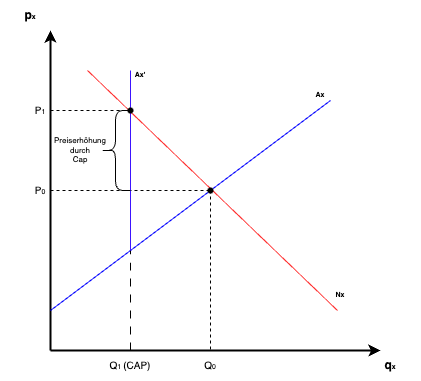
\includegraphics[width=0.8\textwidth]{Bilder/supply_demand_ets.png} 
	\caption{Angebot und Nachfrage von Emissionszertifikaten mit CAP (vgl. \cite{pettinger.2017})}
	\label{fig:supply_demand_ets}
\end{figure}

\begin{figure}[ht]
	\centering
	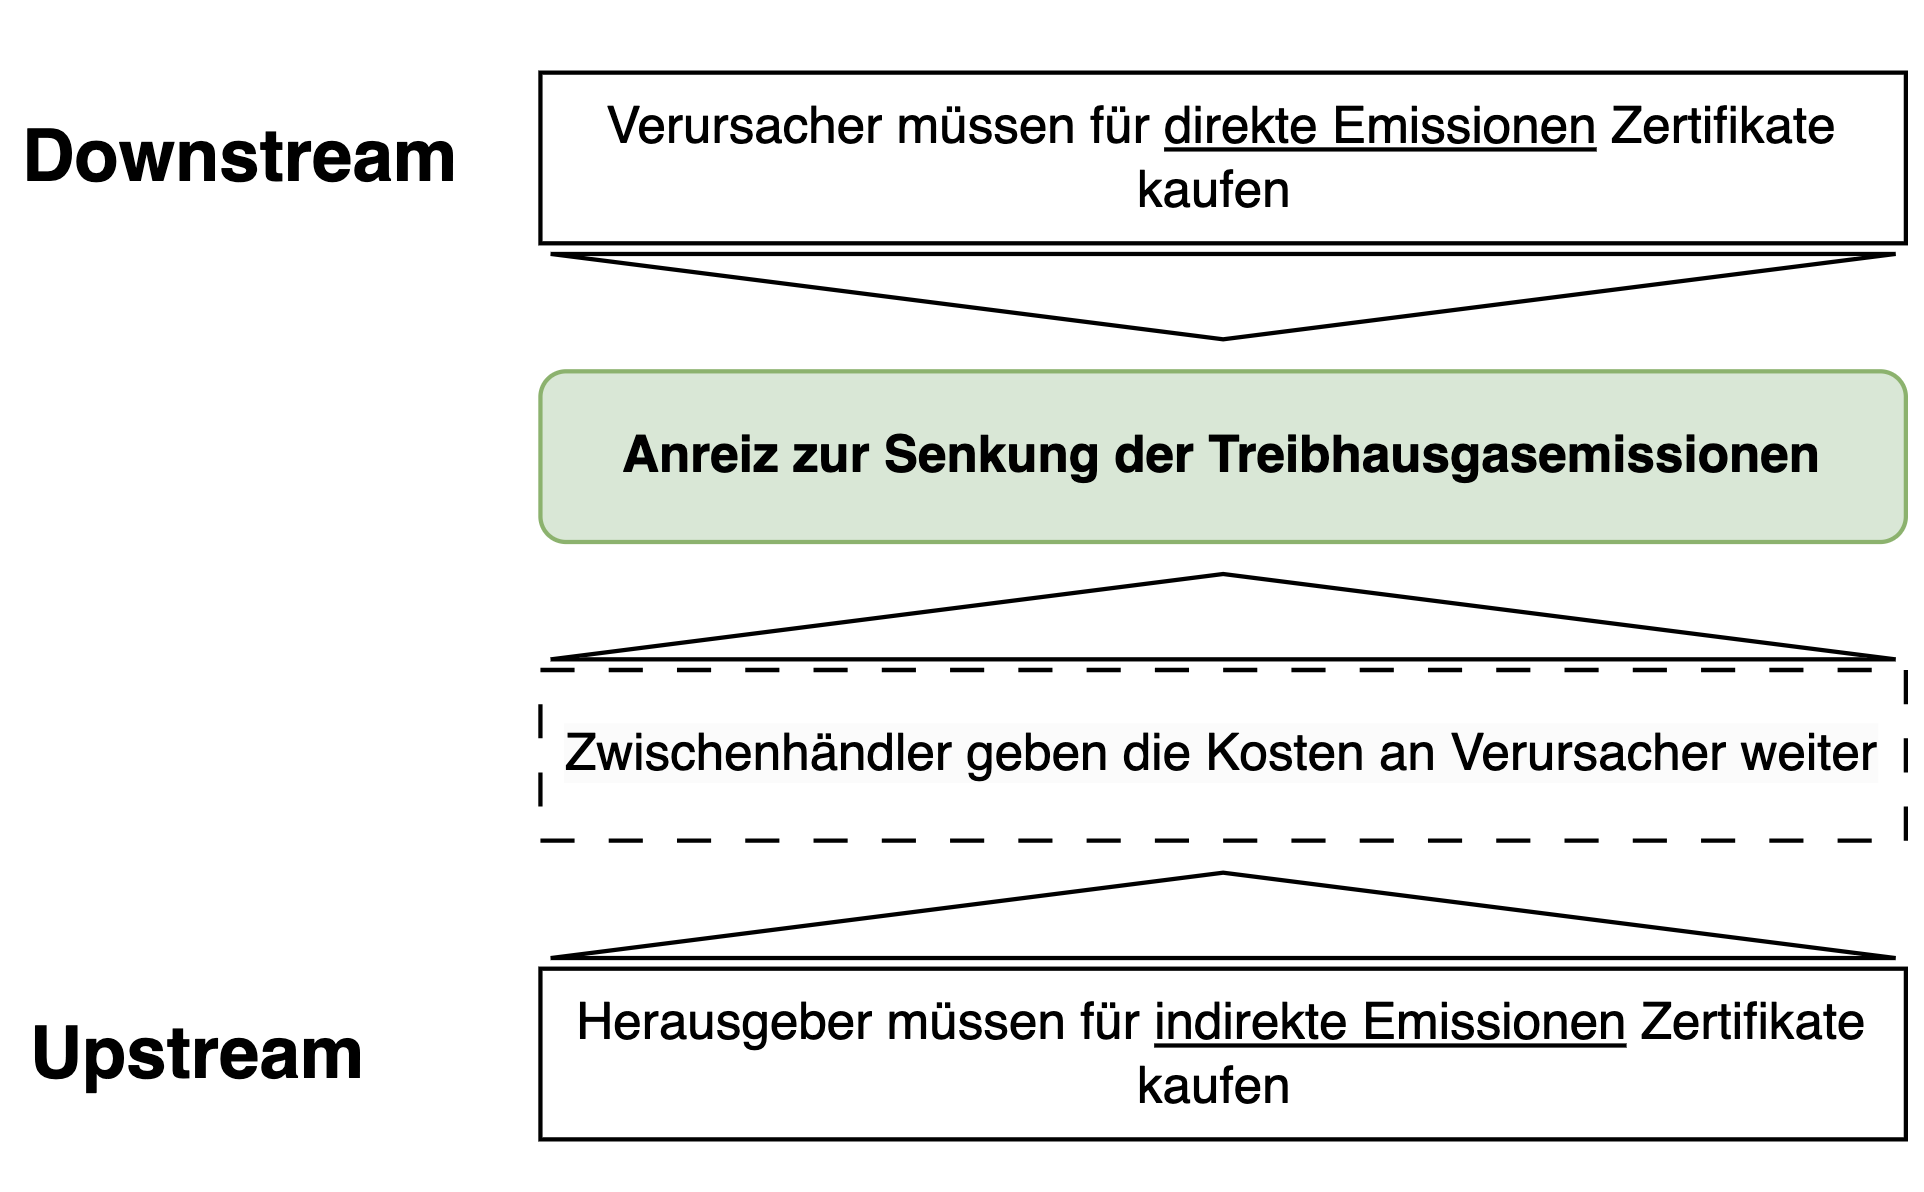
\includegraphics[width=0.8\textwidth]{Bilder/up_and_downstream_ets.png} 
	\caption{Anreize für Verursacher über Upstream- und Downstream-Systeme (vgl. \cite{dehst.2023})}
	\label{fig:up_and_downstream_ets}
\end{figure}

\begin{figure}[ht]
	\centering
	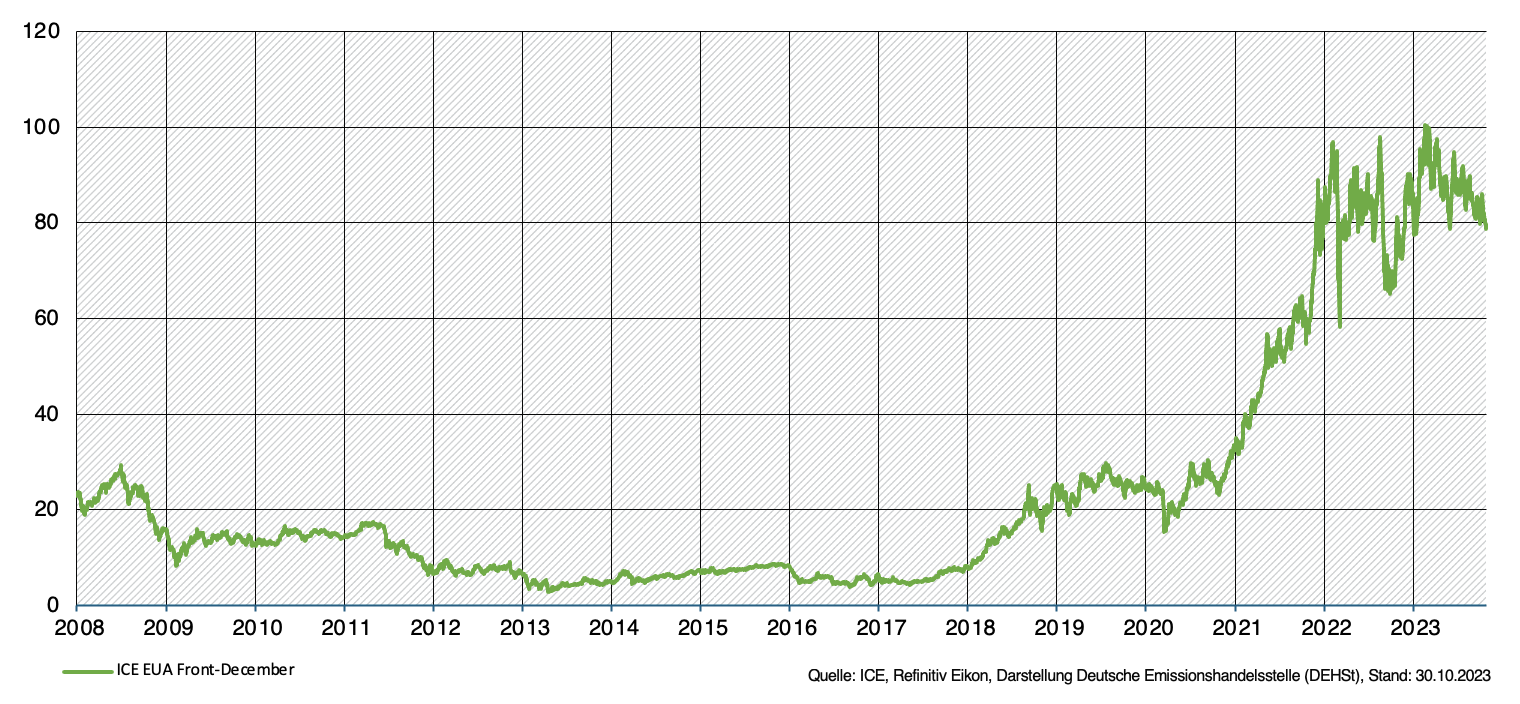
\includegraphics[width=1.0\textwidth]{Bilder/price_co2_eu_ets.png} 
	\caption{Preisentwicklung in € für Emissionsberechtigungen im EU ETS seit 2008 als $CO_2$e-Preis pro Tonne (\cite{dehst.2023})}
	\label{fig:price_co2_eu_ets}
\end{figure}

\begin{figure}[ht]
	\centering
	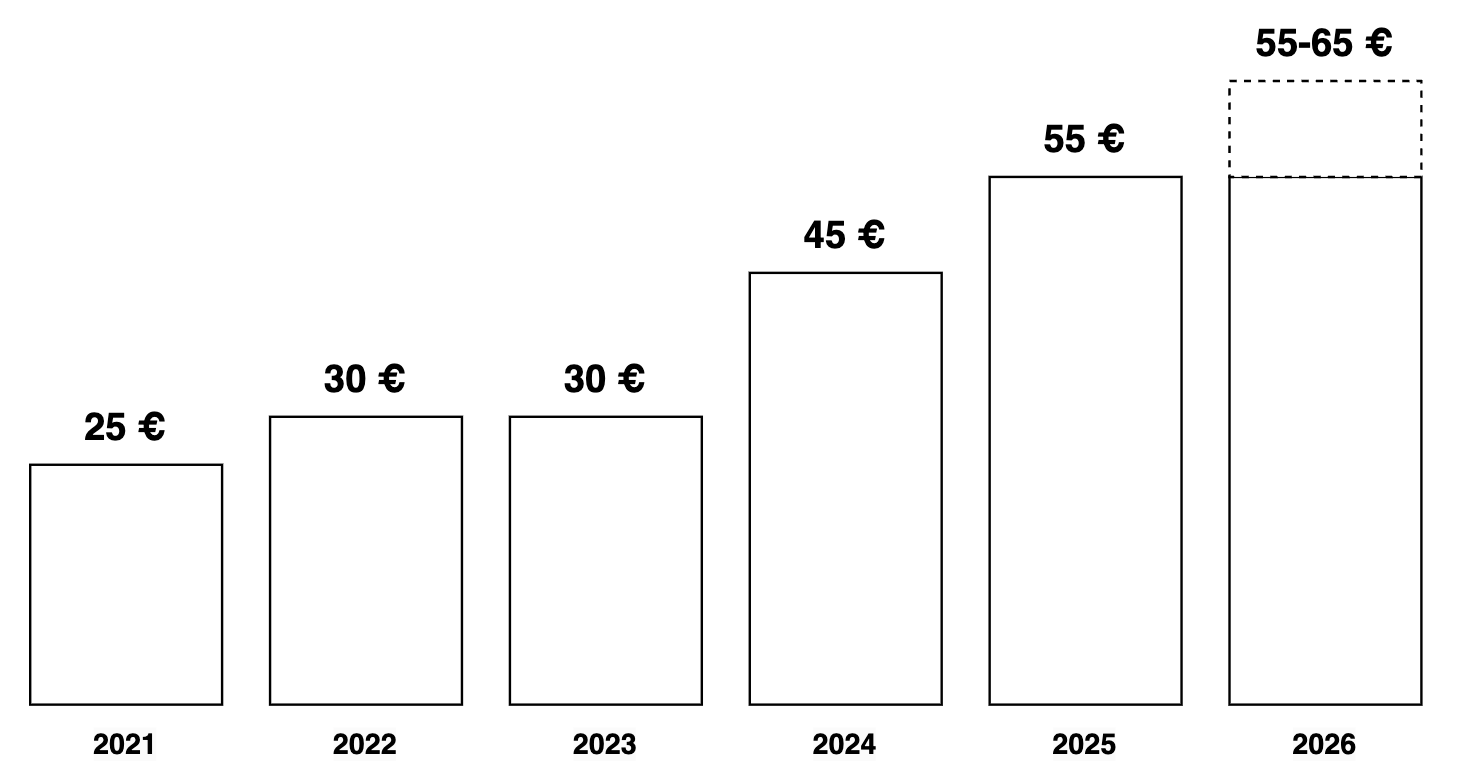
\includegraphics[width=1.0\textwidth]{Bilder/prices_nehs.png} 
	\caption{Preisentwicklung $CO_2$e-Preis pro Tonne für den nEHS (\cite{dehst.2023})}
	\label{fig:prices_nehs}
\end{figure}

% ---- Literaturverzeichnis
\cleardoublepage
\renewcommand*{\chapterpagestyle}{plain}
\pagestyle{plain}
\pagenumbering{Roman}                   % Römische Seitenzahlen
\setcounter{page}{\numexpr\value{savepage}+1}
\printbibliography[title=Literaturverzeichnis]

% ---- Anhang
\appendix
%\clearpage
%\pagenumbering{Roman}  % römische Seitenzahlen für Anhang

\newpage
\end{document}